\documentclass[10pt]{article}
%	options include 12pt or 11pt or 10pt
%	classes include article, report, book, letter, thesis

\usepackage[a4paper,bindingoffset=0.2in,%
left=1in,right=1in,top=0.2in,bottom=0.3in,%
footskip=.15in]{geometry}

\usepackage[T1]{fontenc}
\usepackage[polish]{babel}
\usepackage[utf8]{inputenc}
\usepackage{lmodern}
\usepackage{pgfplots}
\usepackage{graphicx}
\usepackage{amsmath}
\usepackage{subcaption}
\usepackage{multirow}
\usepackage{hyperref}
\usepackage{mathtools}
\newtheorem{hip}{Hipoteza}
\newtheorem{que}{Pytanie}
\newtheorem{wn}{Wniosek}
\newtheorem{wyd}{Zadanie}
\title{Algorytmy numeryczne}
\author{Zadanie 4 \\ Dawid Bińkuś \& Oskar Bir \& Mateusz Małecki\\grupa 1 tester-programista}
\date{13 Styczeń 2019}
\newcommand{\expnumber}[2]{{#1}\mathrm{e}{#2}}
\begin{document}
\maketitle 
\section{Aproksymacja}
Sprawozdanie prezentuje analizę aproksymacji dla problemu określonego w zadaniu 3.
W tym celu, zastosowana została aproksymacja dla metod testowanych w zadaniu 3:
\begin{itemize}
	\item Metoda Gaussa (PG\label{PG}) - wielomian 3-go stopnia,
	\item Metoda Gaussa z drobną optymalizacją dla macierzy rzadkich (SPG\label{SPG}) - wielomian 2-go stopnia,
	\item Metoda Gaussa-Seidela (GS\label{GS}) przy założonej dokładności 1e-10 - wielomian 2-go stopnia,
	\\\\Oraz dodatkowo:
	\item Metoda zaimplementowana w oparciu o macierze rzadkie (S\label{S}) - wielomian 1 stopnia (wykonane za pomocą LUDecomposition z biblioteki Apache Commons Math\footnote{\url{http://commons.apache.org/proper/commons-math/javadocs/api-3.6/overview-summary.html}})
\end{itemize}
Program na potrzeby analizy problemu został napisany w języku Java.
Ilość agentów oznaczana jest jako $N$
\section{Próbka pomiarów czasu}
\subsection{Zakres testów}
Na potrzeby wyliczenia funkcji aproksymacyjnej dla każdej z metod, wykonane zostały testy dla $N = 15,16,...,60$, co przy $N = 60$ odpowiada liczbie około 2000 równań. Dla mniejszej ilości agentów testy wydajnościowe zostały wykonane kilka razy dla uśredniania wyniku.
\subsection{Wyniki}
Wyniki zostały zamieszczone w pliku \href{run:./files/wyniki.csv}{csv}
\section{Aproksymacja średniokwadratowa dyskretna}
Za pomocą aproksymacji średniokwadratowej dyskretnej, wygenerowane zostały wielomiany dla każdego typu pomiarów. Prezentują się one w sposób następujący:
\begin{enumerate}
	\item Generowanie macierzy:
	\begin{enumerate}
		\item $(\expnumber{2.3350439175615983}{-11})x^3 -(\expnumber{3.73562735299031}{-8}) x^2 + (\expnumber{3.927924861861045}{-5}) x^1 -0.006632202623758287$ dla \ref{PG},
		\item $0.026544550834587136 x^1 -12.310426442549858$ dla S (wariant dla wielomianu stopnia 1, $m=1$),
		\item $(\expnumber{1.1160411337156506}{-8})x^3 - (\expnumber{1.138102839915528}{-5})x^2 + 0.006355108980340516 x^1 \\-0.9349542064725634$ dla S (wariant dla wielomianu stopnia 3, $m=3$)
		\item $(\expnumber{3.905262387830365}{-8})x^2 -(\expnumber{2.5264926661242525}{-5})x^1 + 0.006283510185750934 x^0$ dla SPG,
		\item $(\expnumber{5.486623477461811}{-8})x^2 - (\expnumber{5.4389374355751846}{-5}) x^1 + 0.014501100847044942$ dla GS.
	\end{enumerate}
	\item Rozwiązywanie układu równań:
	\begin{enumerate}
		\item $(\expnumber{2.1592223868228134}{-8})x^3 - (\expnumber{3.716638790505861}{-5})x^2 + 0.023672650455756852x^1 \\-3.8108135102259824$ dla PG,
		\item $(\expnumber{1.583603905695412}{-4})x^1 -0.06429601760699291$ dla S,
		\item $(\expnumber{1.3001654605220337}{-6})x^2 - 0.0014560130726117273x^1 + 0.3507906257127139$ dla SPG,
		\item $(\expnumber{2.3048124134271384}{-5})x^2 - 0.020571995359005252x^1 + 4.514786569835568$ dla GS.
	\end{enumerate}
\end{enumerate}
\begin{figure}[h]
	\caption{Wykresy reprezentujące czas wykonania i błędy bezwzględne zaimplementowanych algorytmów \label{Rys1}}
	\begin{subfigure}{0.3\textwidth}
		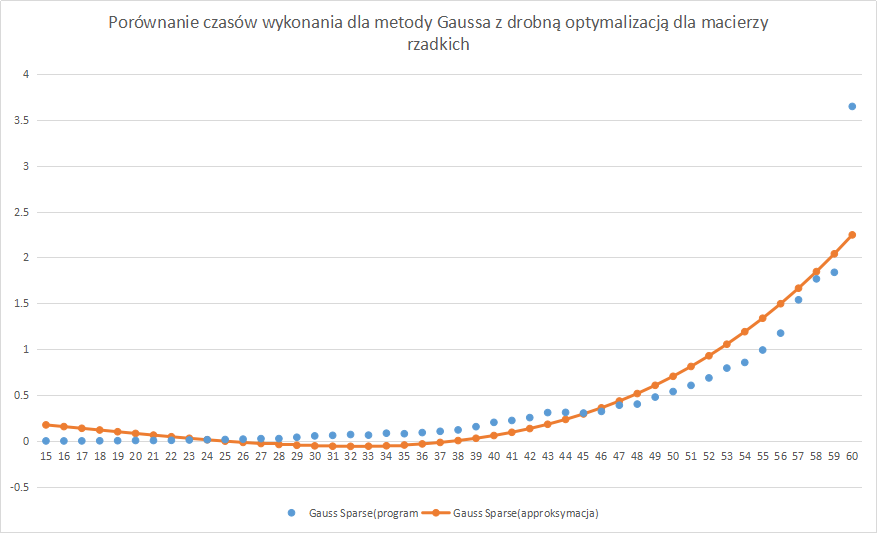
\includegraphics[width=\textwidth]{img/Exec/e1.png}
		\caption{ \label{Rys1a}}
	\end{subfigure}
	\begin{subfigure}{0.3\textwidth}
		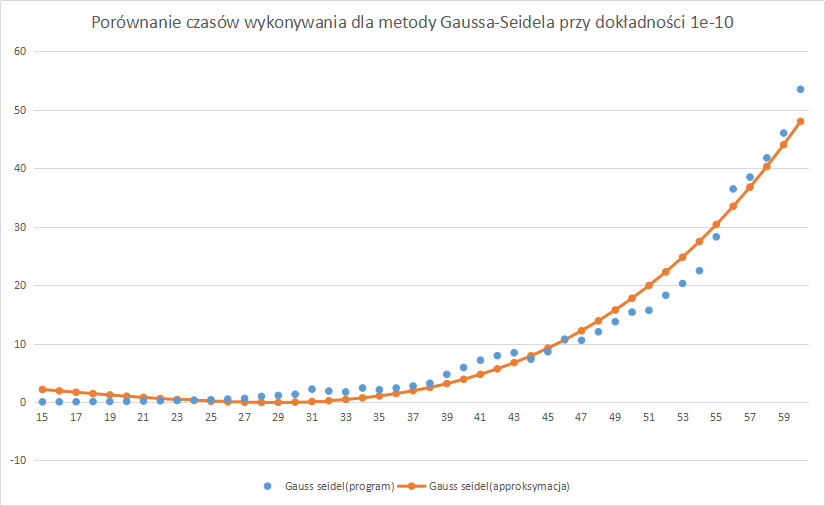
\includegraphics[width=\textwidth]{img/Exec/e2.png}
		\caption{ \label{Rys1b}}
	\end{subfigure}
	\begin{subfigure}{0.3\textwidth}
		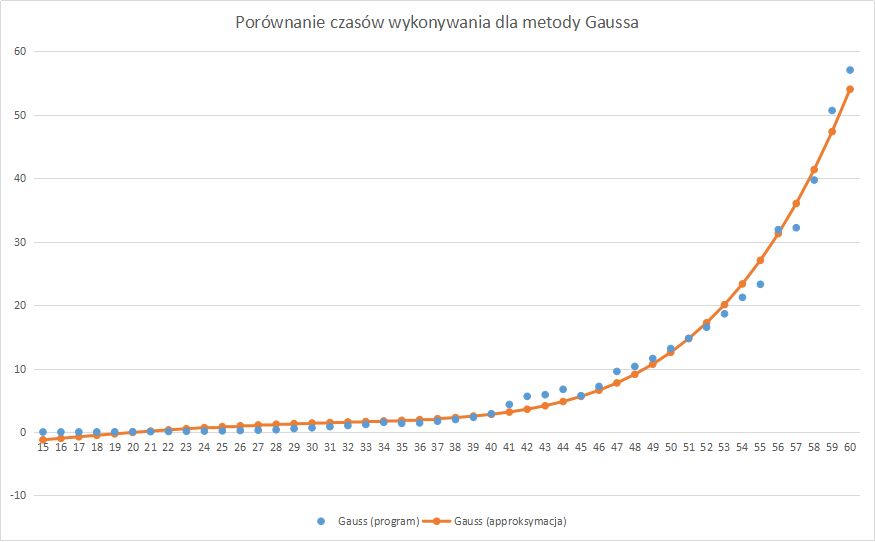
\includegraphics[width=\textwidth]{img/Exec/e3.png}
		\caption{ \label{Rys1c}}
	\end{subfigure}
	\begin{subfigure}{0.3\textwidth}
		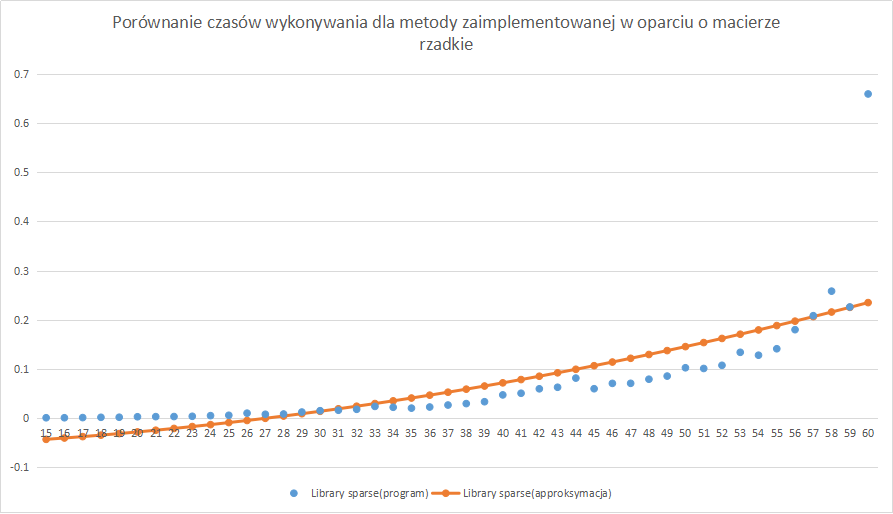
\includegraphics[width=\textwidth]{img/Exec/e4.png}
		\caption{ \label{Rys1d}}
	\end{subfigure}
	\begin{subfigure}{0.3\textwidth}
		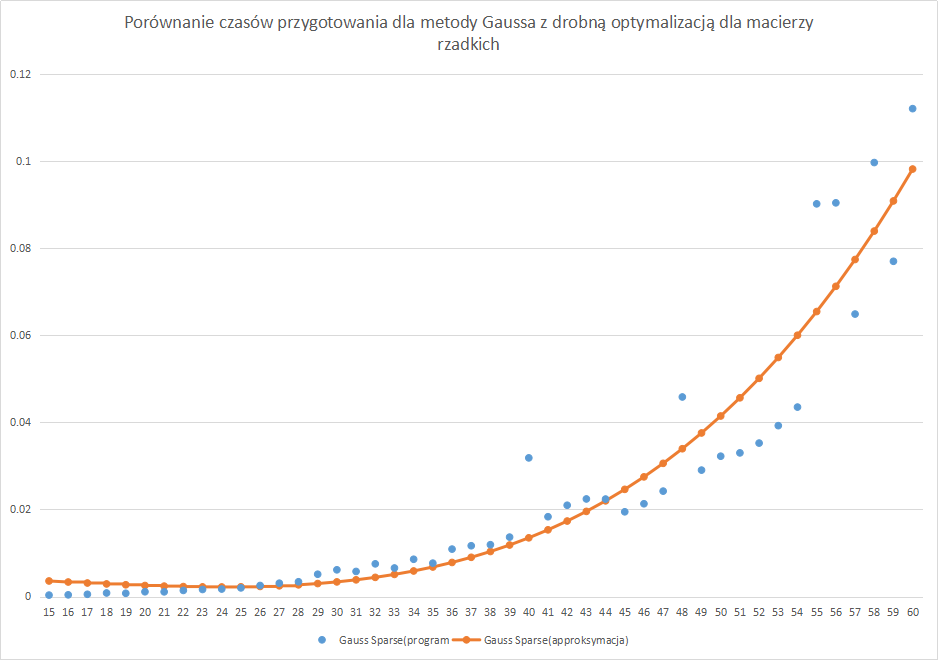
\includegraphics[width=\textwidth]{img/Prep/wyk1.png}
		\caption{ \label{Rys1e}}
	\end{subfigure}
	\begin{subfigure}{0.3\textwidth}
		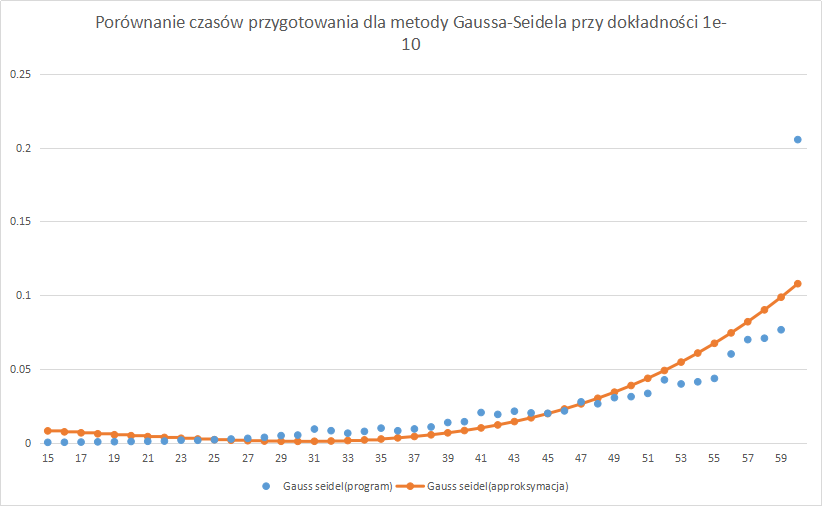
\includegraphics[width=\textwidth]{img/Prep/wyk2.png}
		\caption{ \label{Rys1f}}
	\end{subfigure}
		\begin{subfigure}{0.3\textwidth}
		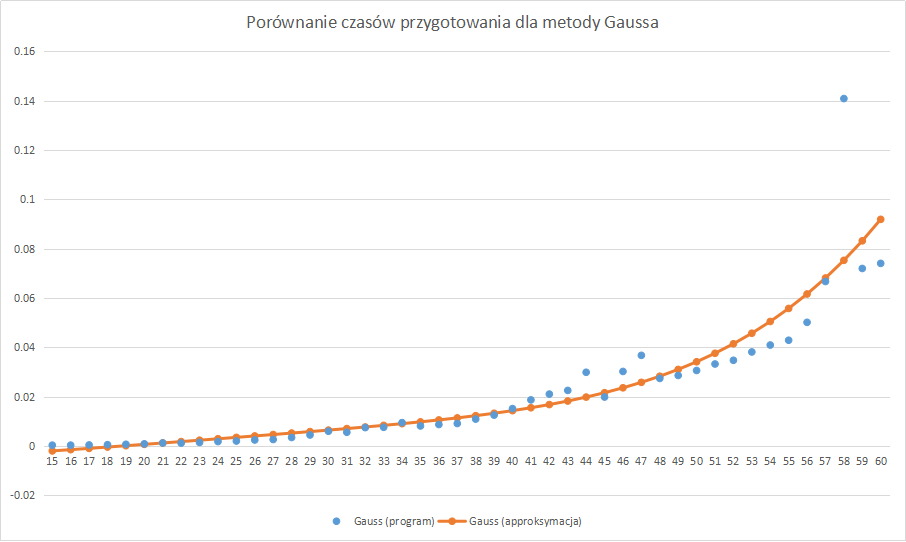
\includegraphics[width=\textwidth]{img/Prep/wyk3.png}
		\caption{ \label{Rys1g}}
	\end{subfigure}
	\begin{subfigure}{0.35\textwidth}
		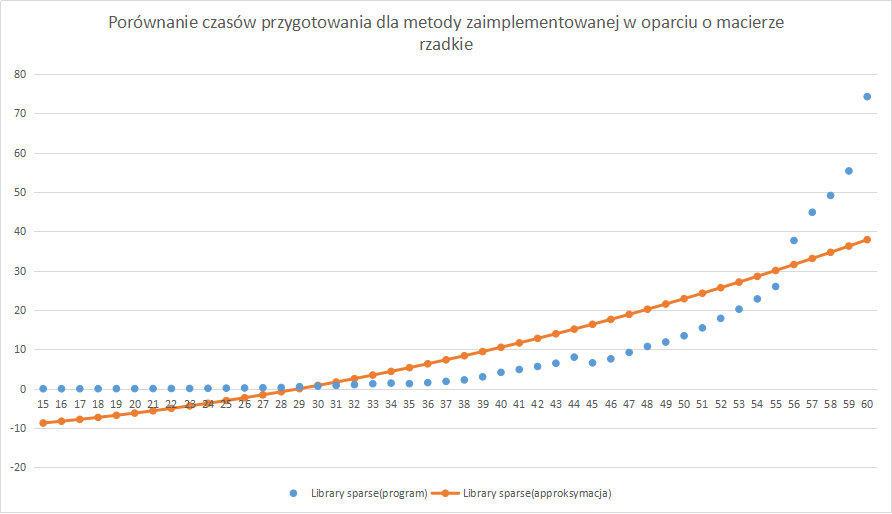
\includegraphics[width=\textwidth]{img/Prep/wyk4.png}
		\caption{ \label{Rys1h}}
	\end{subfigure}
	\begin{subfigure}{0.35\textwidth}
		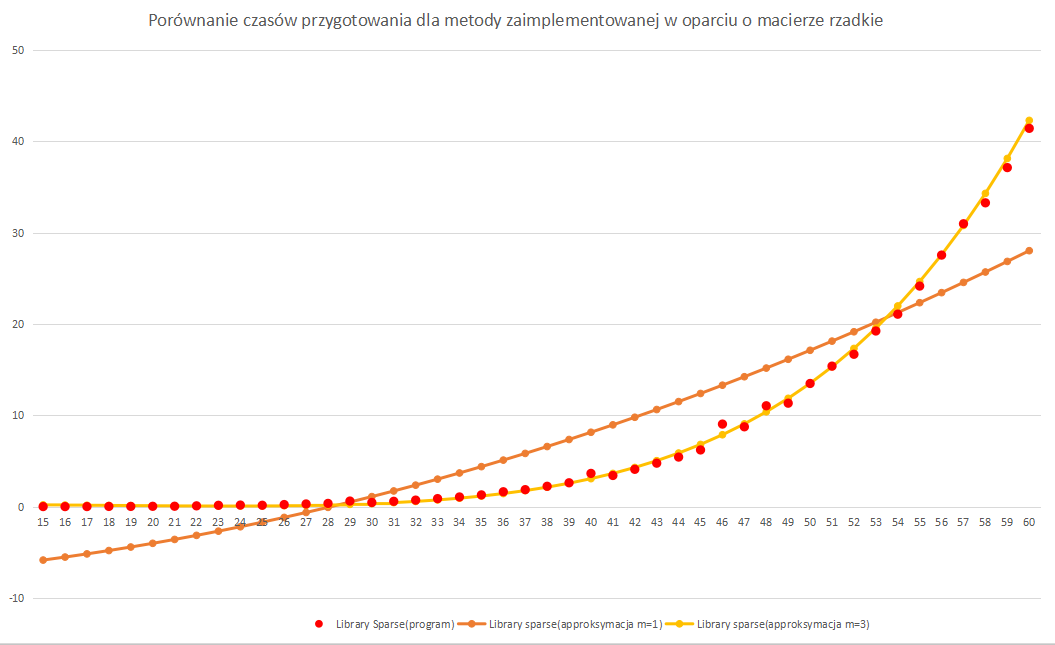
\includegraphics[width=\textwidth]{img/Prep/wyk5.png}
		\caption{ \label{Rys1i}}
\end{subfigure}
\end{figure}
\subsection{Poprawność uzyskanego rozwiązania}
\begin{center}
	\begin{tabular}{|l|l|l|}
		\hline
		\multicolumn{3}{ |c| }{Błąd aproksymacji} \\
		\hline
		Metoda & Wariant & Błąd aproksymacji[s]\\
		\hline
		\multirow{2}{*}{PG} & Obliczanie & $87.52296395468811$ \\
		& Generowanie & $0.0056371667465691345$ \\
		\hline
		\multirow{2}{*}{SPG} & Obliczanie & $2.932007861300984$\\
		& Generowanie & $0.0035357258834377552$\\
		\hline
		\multirow{2}{*}{GS} & Obliczanie & $204.23823436655252$ \\
		& Generowanie & $0.013028009281415509$\\
		\hline
		\multirow{3}{*}{S} & Obliczanie & $0.2257609275320777$ \\
		& Generowanie $m=1$ & $3727.8124913151905$\\
		& Generowanie $m=3$ & $26.142413480394573$\\
		\hline
	\end{tabular}
\end{center}
Jak widać na załączonych wykresach \ref{Rys1} oraz tabeli powyżej prezentującej błąd aproksymacji, w większości przypadków funkcja aproksymująca poprawnie wylicza kolejne czasy wykonywania algorytmu. Wyjątkiem jest funkcja dla generowania w metodzie S. 
\section{Ekstrapolacja}
\section{Próba obliczenia}
\section{Podział pracy}
\centering
\begin{tabular}{| p{4.4cm} | p{4.4cm} | p{4.4cm} |}
	\hline
	\textbf{Dawid Bińkuś} & \textbf{Oskar Bir} & \textbf{Mateusz Małecki} \\ \hline
	Praca nad strukturą projektu. & Analiza algorytmu Gaussa oraz implementacja wariantu G & Implementacja typu własnej precyzji \\ \hline
	Przygotowanie sprawozdania & Przygotowanie testów i ich uruchomienie & Operacje na macierzach\\ \hline
	Implementacja algorytmu Gaussa w wariantach PG i FG & Analiza danych oraz określenie czasu pracy typu Fraction & Praca nad strukturą projektu \\ \hline
	Implementacja generycznej klasy MyMatrix & Przygotowanie wykresów końcowych & Implementacja generycznej klasy MyMatrix \\ \hline	
	\end{tabular}
\end{document}